\chapter{Results}

\begin{figure}[ht!]
	\centering
	\scalebox{1.5}{\input{LIMB.pdf_tex}}
	\label{fig:LIMB}
	\caption{Schematic of measurement and analysis geometry, not to scale.
		The stationary satellite, at a constant height $h_\text{sat}$ above  Earth, takes $m$ measurements.
		The red dashed lines show the line-of-sight from the satellite for each measurement, defining the line $\Gamma_j$ from the satellite with limb height $\ell_j$, $j=1,2,\ldots,m$ (not shown).
		Between $h_0 = 10$km and $h_{n} = 38$km, the stratosphere is discretized into $n$ layers as illustrated by the solid green lines.}
\end{figure}

\begin{itemize}
	\item explain set up of satellite
\end{itemize}

\section{Simulate Data}
In this work we simulate data according to a temperature pressure and ozone profile.
We follow the U.S. standard atmosphere, 1976 \cite{} and the HITRANonline \cite{} database to calculate measurements.


\subsection{Ozone}
\begin{figure}[ht!]
	\centering
	%\scalebox{1}{\input{TrueO3.pdf_tex}}
	\caption{We take the ozone profile from \cite{}, relate pressure and height and discretize according to the source.
		This will serve as our true Ozone profile.}
	\label{fig:nter-label}
\end{figure}
From \cite{} we choose a relatively smooth ozone profile, where each ozone volume mixing ratio corresponds to a distinct pressure values.
Up until $86$km we can relate pressure $p$ and geometric height $h$ through the hydrostatic equation
\begin{align}
	\text{d} \ln p= \frac{\text{d}p}{p} = \frac{- g M}{R^* T} \text{d} h \, ,
\end{align}
with the universal gas consant $R^* \approx 8.314  \, \text{N m} / \text{mol} / \text{K}$ and $M = M_0 \approx 28.97 \, \text{kg}/\text{mol}$ for altiudes below 79km \cite{}.
At altitude $h$ the gravitational constant
\begin{align}
	g = g_0 \Bigg( \frac{r_0}{r_0 + h} \Bigg) \, ,
\end{align}
with $r_0 \approx 6356 \, \text{km}$ (also known as the polar radius of the earth) and $g_0 \approx 9.81 \text{m}/\text{s}^2$ and \cite{}.
In the discretized case, we approximate $g(h) \approx g(h_i) $ at $h_i = \Delta h + h_{i-1}$ for the $ith$ layer in the atmosphere.

\subsection{Pressure}
We parametrize the pressure by fitting two exponentials to the pressure values $p$ related to the height $h$ by Eq. \ref{}.
\begin{figure}[ht!]
	\centering
	%\scalebox{1}{\input{TruePress.pdf_tex}}
	\caption{In green the true pressure profile, where we fit two exponential to it.
		Above $h_{p,0}$ the gradient of the epxonetinal is $a_{p,1}$ and below $a_{p,0}$.
		We have a $p_0$ wehere those two expontentials meet}
	\label{fig:nter-label}
\end{figure}
The pressure function,
\begin{align}
	p(h) = \begin{cases*}
		\exp{ \{ -a_{p,0} \,  (h - h_{p,0} ) \} } \,  p_0, & \text{$h < h_{p,0}$}\\\
		p_0,  & \text{$h = h_{p,0}$}\\
		\exp{ \{ -  a_{p,1} \, (h - h_{p,0} )  \} \, p_0}, & \text{$h > h_{p,0}$}\
	\end{cases*} \, ,
\end{align}
is depending on four different parameters, the gradient $a_{p,1}$ above $h_{p,0}$ and $a_{p,0}$ below $h_{p,0}$.
Both exponentials meet at $p_0$.


\subsection{Temperature}
The temperature is taken from \cite{}.
\begin{figure}[ht!]
	\centering
	%\scalebox{1}{\input{TrueTemp.pdf_tex}}
	\caption{True temperature profile, in the altitude of interest.
		The gradients $a_0,a_1,a_2,a_3,a_4$ and the corresponding height $h_0,h_1,h_2,h_3,h_4,h_5$ as well as the temperature $T_0$ at $h = 0$ are taken from the us standard atmosphere and parametrize the temperature profile.}
	\label{fig:nter-label}
\end{figure}
We can formulate a temperature function
\begin{align}
	T(h) = \begin{cases*}
		T_0 & \text{$h = 0$}\\
		a_0 h  + T_0, & \text{$0 \leq h < h_{0}$}\\
		a_0 h_0  + T_0  , & \text{$h_{0} \leq  h < h_{1}$}\\
		a_1 (h -h_1)+ a_0 h_0 + T_0 , & \text{$h_{1} \leq h < h_{2}$}\\
		a_2 (h -h_2) + a_1 (h_2 - h_1) + a_0 h_0  + T_0, & \text{$h_{2} \leq h < h_{3}$}\\
		a_2  (h_3 - h_2) +  a_1 (h_2 - h_1) + a_0 h_0 + T_0, & \text{$h_{3} \leq h < h_{4}$}\\
		a_3 (h -h_4) + a_2  (h_3 - h_2) + a_1 (h_2 - h_1)+ a_0 h_0 + T_0, & \text{$h_{4} \leq h < h_{5}$}\\
		a_4 (h -h_5) + a_3 (h_4 - h_4)+ a_2  (h_3 - h_2) + a_1 (h_2 - h_1)+ a_0 h_0 + T_0, & \text{$h_{5} \leq h < 84.852\text{km}$}
	\end{cases*} 
\end{align}
depending on 12 parameters with values provided by \cite{}, also see table \ref{}.
We set this as our true temperature profile and refer to \cite{} for temperature values above $79 \,\text{km}$.


\subsection{Source}
We calculate the source function $B(\nu, T)$ and the absorption constant $ k(\nu, T)$ as follows.

For one species at one specific wave-number the weighted absorption constant becomes
\begin{align}
	\overline{k(\nu, T, r)}    = \sum_{m=1}^{molec} k_m(\nu, T) x_m(r) =  k(\nu, T) x(r) \, ,
\end{align}
with the volume mixing ratio of ozone $x(r)$ at location $r$. 
The absorption constant
\begin{align}
	k(\nu, T) = L(\nu, T_{\text{ref}}) \frac{Q(T_{\text{ref}})}{Q(T)} \frac{ \exp{\{ - c_2 E^{\prime \prime} / T\}} }{\exp{\{ - c_2 E^{\prime \prime} / T_{\text{ref}} \}}} \frac{ 1- \exp{\{ - c_2 \nu  / T \}} }{1 - \exp{\{ - c_2 \nu / T_{\text{ref}} \}}}
\end{align}
is depend on the line intensity $L(\nu, T_{\text{ref}}$ at reference temperature $T_{\text{ref}} =296K $, the lower-state energy of the transition $ E^{\prime \prime} $, the second radiation constant $c2=1.4387769\text{cmK}$ all provided by \cite{}.
Since we only consider one transition namely the lower-state one the partition function becomes
\begin{align}
	Q(T )= g^{\prime \prime} \exp{\{ - \frac{ c_2 E^{\prime \prime} }{T}\}} \, ,
\end{align}
with the the statistical weight $ g^{\prime \prime}$ (also called the degeneracy factor), see \ref{}.
M. Šimečková, D. Jacquemart, L. S. Rothman, R. R. Gamache, and A. Goldman, "Einstein A-coefficients and statistical weights for molecular absorption transitions in the HITRAN database", J. Quant. Spectrosc. Radiat. Transfer 98, 130-155 (2006)

Under the assumption of local thermodynamic (LTE) equilibrium t source function is given by the black body radiation
\begin{align}
	B(\nu,T)   = \frac{2 h c^2 \nu^3}{\exp{\{\frac{hc\nu}{k_B T}\}}-1}\, ,
\end{align}
with Planck's constant $h$, velocity of light $c$ and Boltzmann's constant $k_B$ \cite{}.




\section{Bayesian Model and prior analysis}


\subsection{DAG}

\begin{figure}[thb!]
	\centering
	\begin{tikzpicture}
		\node[roundnode2] at (-4.5,6.5) (Q)     {$\bm{Q}$};
		\node[roundnode2] at (-3,5) (x)     {$\bm{x}$};
		\node[roundnode2] at (-1,4) (A)    {$\bm{A}_{NL}$};
		\node[roundnode2] at (-1,2.5) (u)    {$\bm{u}$};
		\node[rectnode] at (-1,1) (y)    {$\bm{y}$};
		\node[roundnode2] at (-5.25,4.5) (S)    {$\bm{\Sigma}$};
		\node[roundnode2] at (-6.5,6.25) (s)    {$\gamma$};
		\node[roundnode2] at (-5.5,8) (d)    {$\delta$};
		\node[roundnode2] at (3,6.5) (t)     {$\bm{T}$};
		\node[roundnode2] at (-1,6.5) (p)     {$\bm{p}$};
		\node[roundnode2] at (1,5) (pt)     {$\bm{p}/\bm{T}$};
		\node[roundnode2] at (0,8) (b1)    {$b_1$};
		\node[roundnode2] at (1,8) (b2)    {$b_2$};
		\node[roundnode2] at (-2,8) (h1)    {$h_0$};
		\node[roundnode2] at (-1,8) (p0)    {$p_0$};
		\node[roundnode2] at (2.25,8) (ht)    {$\bm{h_T}$};
		\node[roundnode2] at (3.25,8) (ct)    {$\bm{c_T}$};
		\node[roundnode2] at (4.25,8) (at)    {$\bm{a_T}$};
		
		%Lines
		\draw[->, mydotted, very thick] (S.south east) -- (y.west);
		\draw[->, very thick] (s.south) -- (S.north west);
		\draw[->, very thick] (u.south) -- (y.north);
		\draw[->, mydotted, very thick] (A.south) -- (u.north);
		\draw[->, mydotted,  very thick] (x.south east) -- (A.west);
		\draw[->, very thick] (p.south east) -- (pt.north west);
		\draw[->, very thick] (t.south west) -- (pt.north east);
		\draw[->,  mydotted, very thick] (pt.south west) -- (A.east);
		\draw[->, very thick] (h1.south) -- (p.north west);
		\draw[->, very thick] (p0.south) -- (p.north);
		\draw[->, very thick] (b1.south) -- (p.north east); 
		\draw[->, very thick] (b2.south) -- (p.east); 
		
		\draw[->, very thick] (d.south) -- (Q.north west); 
		
		\draw[->, very thick] (Q.south east) -- (x.north west); 
		\draw[->, very thick] (ht.south) -- (t.north west);
		\draw[->, very thick] (ct.south) -- (t.north);
		\draw[->, very thick] (at.south) -- (t.north east);
		
		
		\node[align=center] at (0.25,3.95) (f3) {$\approx \bm{M A}_L$};
		
	\end{tikzpicture} 
\end{figure}

\begin{align}
	\bm{Q}= \delta \bm{L} =
	\delta
	\begin{bmatrix}
		2 & -1 & & &  \\
		-1 & 2 & -1 & &   \\
		& \ddots & \ddots & \ddots &\\ 
		&   & -1 & 6 & -5 \\
		& & & \ddots & \ddots & \ddots  \\ 
		& & & &  -5 & 10 & -5 \\
		& & & & & -5 & 10 
	\end{bmatrix}  
\end{align}

\begin{table}
	\centering
	\begin{tabular}{ |c||c|c|c|c|   }
		\hline
		& &\multicolumn{2}{|c|}{TT bounds}&\\
		\hline
		model parameters& priors&\makecell{lower}& \makecell{upper\\
		}&Context\\
		\hline
		
		$\gamma$ & $\mathcal{T}(1,10^{-10})$ &- &-& $\bm{x}$\\ \hhline{|=||=|=|=|=|}
		$\delta$ &$\mathcal{T}(1,10^{-10})$ & -&-& $\bm{x}$\\ \hline
		%$\gamma$ & $\mathcal{N}(2.58e-9,2.58e-11)$ &2.45e-9&2.7e-9 &$\bm{x}$\\
		%$\delta_0$ &  $\mathcal{N}(0.8e-4,0.75e-5)$& 4e-5 & 1.1e-4&$\bm{x}$\\
		$a_0$ &  $\mathcal{T}(3,1e6)$& 1e-15&1e-5&$\bm{x}$\\ \hline
		$h_0$ &  $\mathcal{N}(31.35,1)$&27 &35&$\bm{x}$\\ \hline
		$h_{p,1}$ &  $\mathcal{N}(34.3,0.5)$& 32.8&35.64&$\bm{p/T}$\\ \hline
		$p_0$ &  $\mathcal{N}(6.5,0.1)$&6.17 &6.73&$\bm{p/T}$\\ \hline
		$b_1$ &  $\mathcal{N}(0.15,0.0051)$& 0.138  &0.167&$\bm{p/T}$\\ \hline
		$b_2$ & $\mathcal{N}(0.13,0.067)$& 0&0.32&$\bm{p/T}$\\ \hline
		$h_{t,0}$ &  $\mathcal{N}(11,0.5)$&9.6 &12.4&$\bm{p/T}$\\ \hline
		$h_{t,1}$ &  $\mathcal{N}(20,3)$&11.6 &28.4&$\bm{p/T}$\\ \hline
		$h_{t,2}$ &  $\mathcal{N}(32,1)$&29.2 &34.8&$\bm{p/T}$\\ \hline
		$h_{t,3}$ &  $\mathcal{N}(47,2)$&41.4 &52.6&$\bm{p/T}$\\ \hline
		$h_{t,4}$ &  $\mathcal{N}(51,2)$&45.4 &56.6&$\bm{p/T}$\\ \hline
		$h_{t,5}$ &  $\mathcal{N}(71,2)$&65.4 &76.6&$\bm{p/T}$\\ \hline
		$a_{t,1}$ &  $\mathcal{N}(-6.5,0.01)$&-6.528 &-6.472&$\bm{p/T}$\\ \hline
		$a_{t,2}$ &  $\mathcal{N}(1,0.01)$&0.972 &1.028&$\bm{p/T}$\\ \hline
		$a_{t,3}$ &  $\mathcal{N}(2.8,0.1)$&2.52 &3.078&$\bm{p/T}$\\ \hline
		$a_{t,4}$ &  $\mathcal{N}(-2.8,0.01)$&-2.828 &-2.772&$\bm{p/T}$\\ \hline
		$a_{t,5}$ & $\mathcal{N}(-2,0.01)$ &-2.028 &-1.972&$\bm{p/T}$\\ \hline
		$t_{0}$ &  $\mathcal{N}(288,2)$& 282.54 &293.75&$\bm{p/T}$\\
		\hline
	\end{tabular}
	\caption{Gaussian $\mathcal{N}(\mu,\sigma)$ and gamma distribution $\mathcal{T}(\alpha = \text{scale}, \beta = \text{rate})$
		Bounds for t and p 2.8 times the variance around the mean
		round pressure approx and  test if would work with previous gamma prior or fix gamma prior with set values}
	\label{tab:1}
\end{table}

\subsection{Prior Modelling}
\begin{itemize}
	\item prior of ozone (picture), with samples drawn from gamma distr
	\item prior of pressure and temperature
\end{itemize}

\subsection{Posterior distributions}
\begin{itemize}
	\item explain where we use MTC and that T/p is spereate
	\item marginal posterior, noise and covarince and perciosn matrix
	\item picture of f and g
	\item taylor expansion
	\item maybe make  metroplis explixit
\end{itemize}


\section{Affine Map}
\begin{itemize}
	\item explicit, why we need ozone porifles, bcause it is faster
\end{itemize}
In this specific case we find the affine map
\begin{align}
	\bm{M} = \begin{bmatrix}
		\text{---} & \bm{M}_0 &   \text{---}  \\
		&  \vdots  & \\
		\text{---}& \bm{M}_j &  \text{---} \\
		&  \vdots  & \\
		\text{---} & \bm{M}_m &   \text{---}
	\end{bmatrix} \, \in \mathbb{R}^{m \times m} ,
\end{align}
with rows $\bm{M}_j$ using a linear solver for
\begin{align}
	W \bm{M}_j^\top \, = V_{j} \, .
\end{align}
Here $V_j$ denotes the $j$th row of  
\begin{align}
	V = \begin{bmatrix}
		\vert&   &  \vert & & \vert \\
		\bm{A}_{NL} (\bm{x}^{(1)} ) &  \cdots& \bm{A}_{NL} (\bm{x}^{(j)} )&  \cdots & \bm{A}_{NL} (\bm{x}^{(m)})  \\
		\vert&   &  \vert & & \vert 
	\end{bmatrix}
\end{align}
and
\begin{align}
	W = \begin{bmatrix}
		\vert&   &  \vert & & \vert \\
		\bm{A}_{L} \bm{x}^{(1)} &  \cdots& \bm{A}_{L} \bm{x}^{(j)} &  \cdots & \bm{A}_{L} \bm{x}^{(m)} \\
		\vert&   &  \vert & & \vert 
	\end{bmatrix}
\end{align}
is a $\mathbb{R}^{m \times m} $ matrix as well as $\bm{A}_{NL}$.
Then the non-linear forward model can be approximated so that
\begin{align}
	\bm{A}_{NL}(\bm{x}) \approx \bm{M A}_L \bm{x}\, .
\end{align}

\subsection{First MTC}
\begin{itemize}
	\item make table with set up for TT and sampling 
\end{itemize}
\begin{figure}[thb!]
	\centering
	\begin{tikzpicture}
		\node[roundnode2] at (-4.5,6.5) (Q)     {$\bm{Q}$};
		\node[roundnode2] at (-3,5) (x)     {$\bm{x}$};
		\node[roundnode2] at (-1,4) (A)    {$\bm{A}_{NL}$};
		\node[roundnode2] at (-1,2.5) (u)    {$\bm{u}$};
		\node[rectnode] at (-1,1) (y)    {$\bm{y}$};
		\node[roundnode2] at (-5.25,4.5) (S)    {$\bm{\Sigma}$};
		\node[roundnode2] at (-6.5,6.25) (s)    {$\gamma$};
		\node[roundnode2] at (-5.5,8) (d)    {$\delta$};
		
		%Lines
		\draw[->, mydotted, very thick] (S.south east) -- (y.west);
		\draw[->, very thick] (s.south) -- (S.north west);
		\draw[->, very thick] (u.south) -- (y.north);
		\draw[->, mydotted, very thick] (A.south) -- (u.north);
		\draw[->, mydotted,  very thick] (x.south east) -- (A.west);
		
		\draw[->, very thick] (d.south) -- (Q.north west); 
		
		\draw[->, very thick] (Q.south east) -- (x.north west); 
		%\node[align=center] at (0,4) (f3) {$= \bm{A}$};
		\node[align=center] at (0.25,3.95) (f3) {$\approx \bm{M A}_L$};
		
	\end{tikzpicture} 
\end{figure}

\subsubsection{Marginal Posterior}


\begin{figure}[ht!]
	\centering
	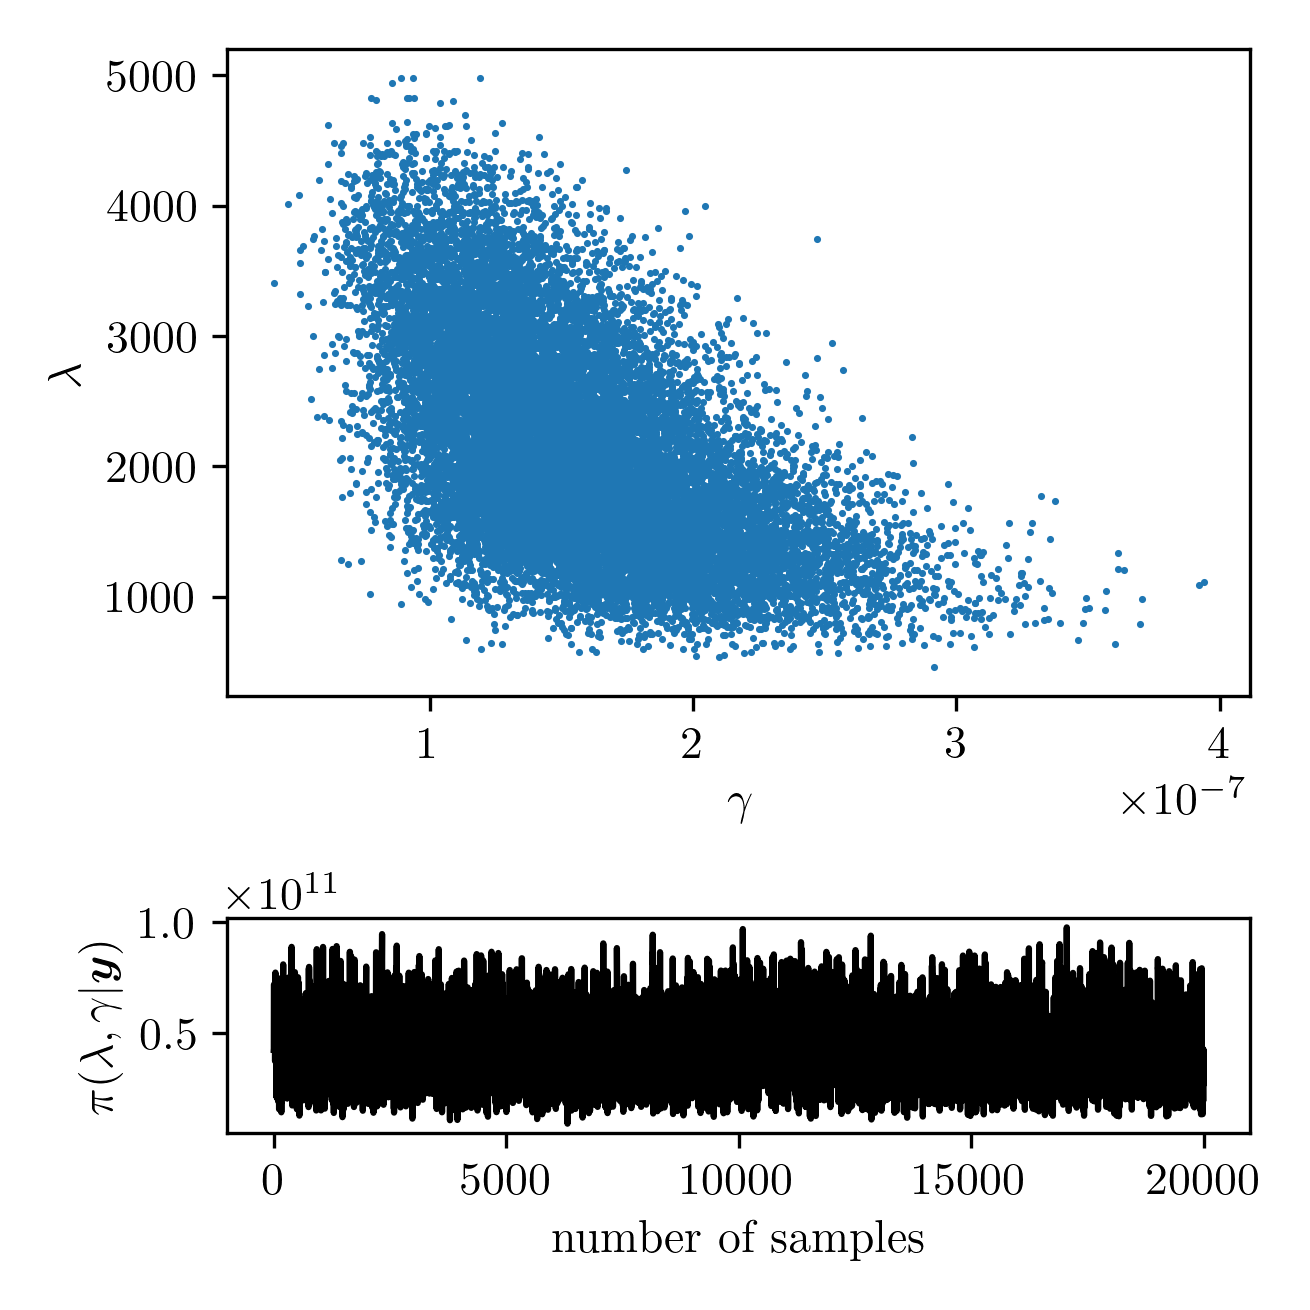
\includegraphics{ScatterplusHisto.png}
	\caption[]{}
	\label{fig:}
\end{figure}

\subsubsection{cinditional osterior Posterior}
\begin{figure}[ht!]
	\centering
	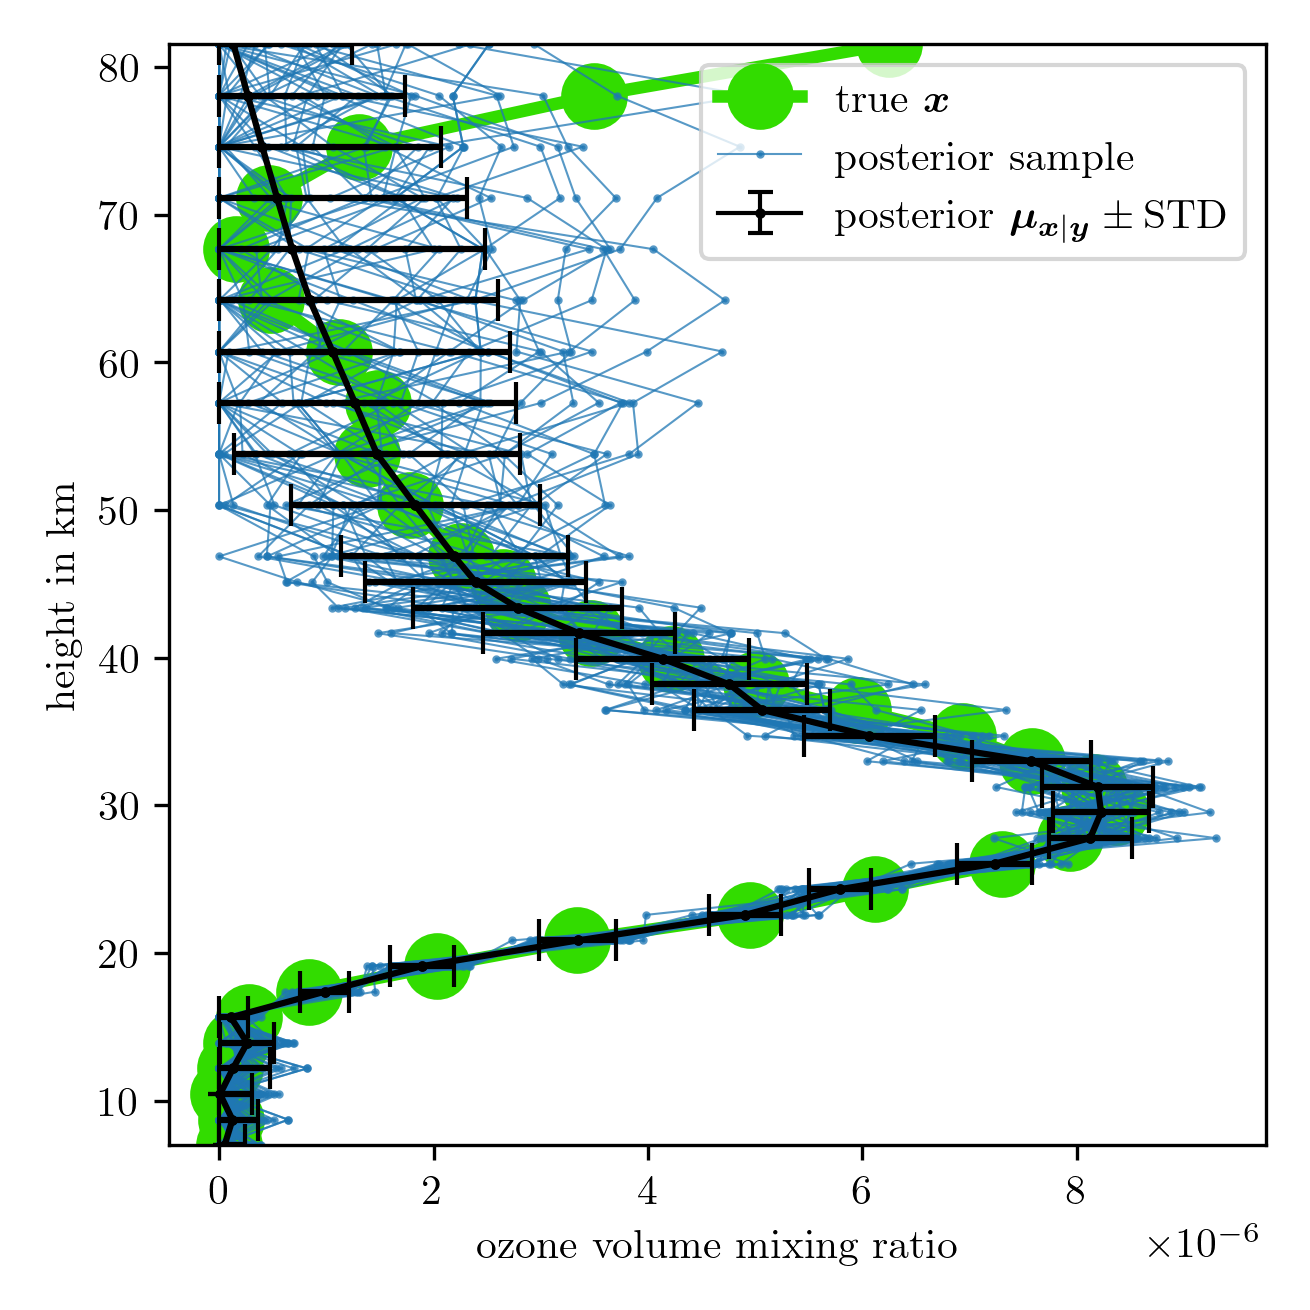
\includegraphics{FirstTestRes.png}
	\caption[]{}
	\label{fig:}
\end{figure}


\subsection{Asses Affine Map}
\begin{figure}[ht!]
	\centering
	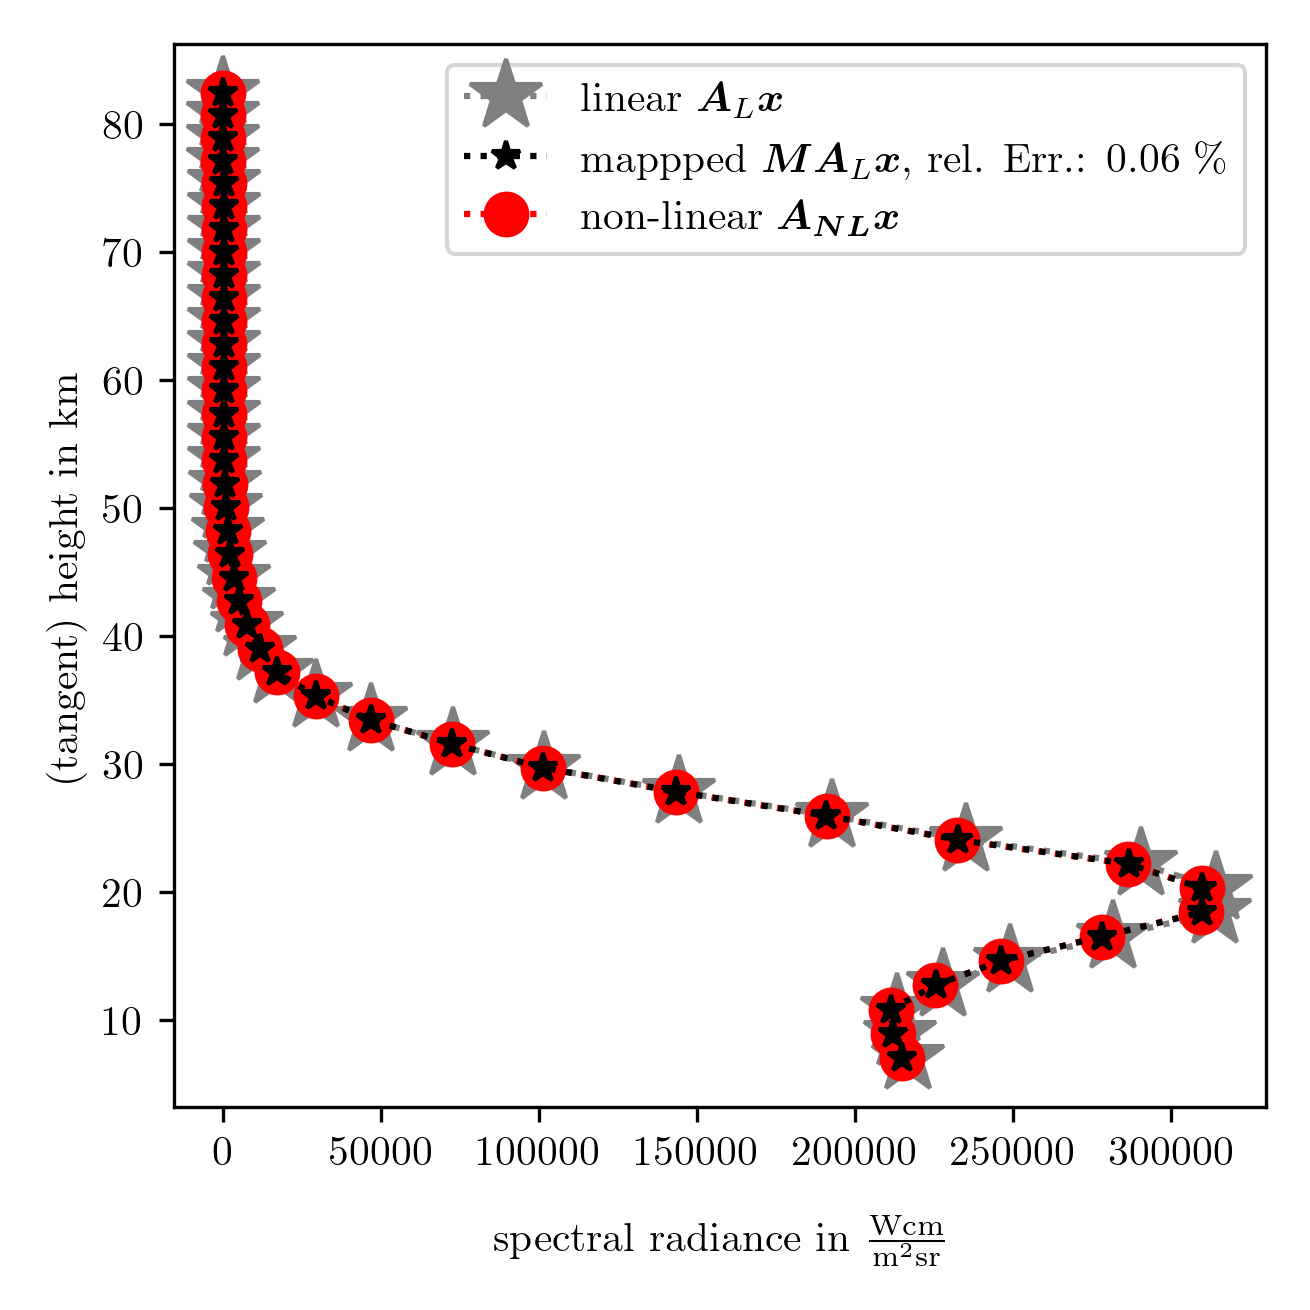
\includegraphics{SampMapAssesment.png}
	\caption[]{}
	\label{fig:}
\end{figure}


\section{Updated Forward map}

\begin{itemize}
	\item updated forward map
		\item do mtc again and then condition on pressure and temperature, samples
\end{itemize}


\section{Ozone Retrieval }
\begin{figure}[ht!]
	\centering
	\includegraphics{secRecRes.png}
	\caption[]{}
	\label{fig:}
\end{figure}

\subsection{Marginal Posterior}
\begin{figure}[ht!]
	\centering
	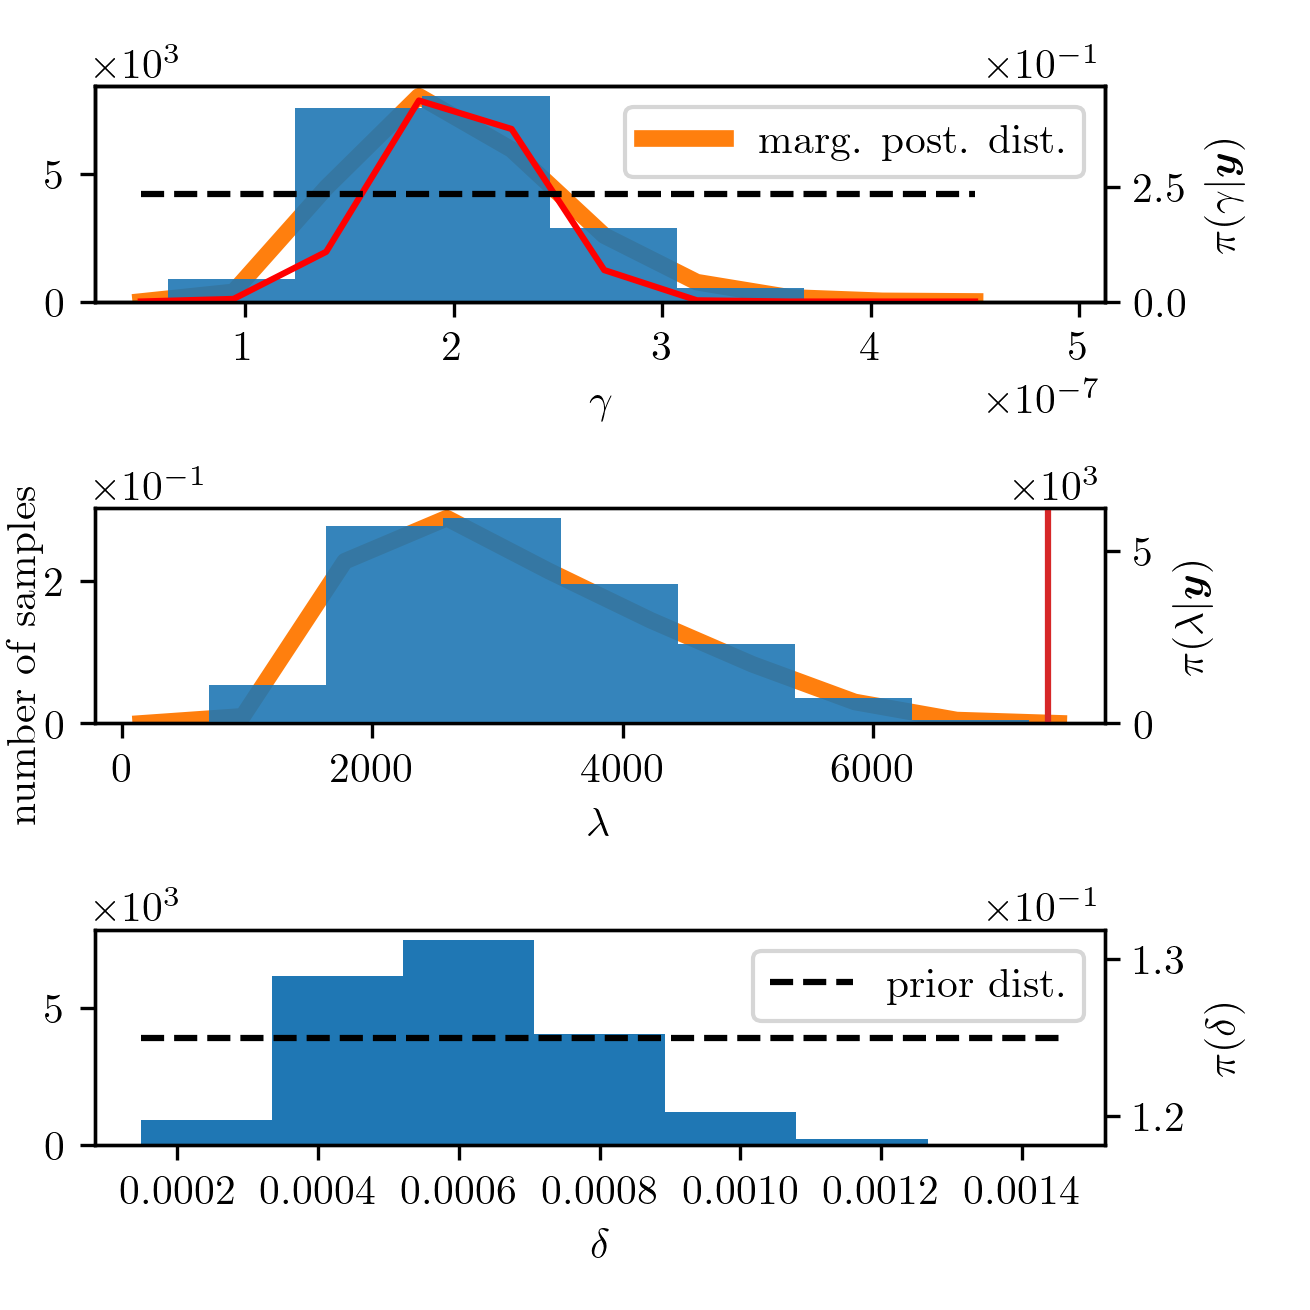
\includegraphics{secSIRTMargMargO3Res.png}
	\caption[]{}
	\label{fig:}
\end{figure}
\subsection{Regularized Solution}
\begin{itemize}
	\item similar to MTC model
	\item picture of L-Curve and samples 
	\item include in reg paraemter in histograms
\end{itemize}

\begin{figure}[ht!]
	\centering
	%\includegraphics{Reg.png}
	\caption[]{}
	\label{fig:}
\end{figure}
\section{Posterior Pressure and Temperature}
\begin{itemize}
	\item make table with set up for TT and sampling 
\end{itemize}
\begin{figure}[thb!]
	\centering
	\begin{tikzpicture}
		
		\node[roundnode2] at (-1,4) (A)    {$\bm{A}_{NL}$};
		\node[roundnode2] at (-1,2.5) (u)    {$\bm{u}$};
		\node[rectnode] at (-1,1) (y)    {$\bm{y}$};
		
		\node[roundnode2] at (3,6.5) (t)     {$\bm{T}$};
		\node[roundnode2] at (-1,6.5) (p)     {$\bm{p}$};
		\node[roundnode2] at (1,5) (pt)     {$\bm{p}/\bm{T}$};
		\node[roundnode2] at (0,8) (b1)    {$b_1$};
		\node[roundnode2] at (1,8) (b2)    {$b_2$};
		\node[roundnode2] at (-2,8) (h1)    {$h_0$};
		\node[roundnode2] at (-1,8) (p0)    {$p_0$};
		\node[roundnode2] at (2.25,8) (ht)    {$\bm{h_T}$};
		\node[roundnode2] at (3.25,8) (ct)    {$\bm{c_T}$};
		\node[roundnode2] at (4.25,8) (at)    {$\bm{a_T}$};
		
		%Lines
		
		\draw[->, very thick] (u.south) -- (y.north);
		\draw[->, mydotted, very thick] (A.south) -- (u.north);
		
		\draw[->, very thick] (p.south east) -- (pt.north west);
		\draw[->, very thick] (t.south west) -- (pt.north east);
		\draw[->,  mydotted, very thick] (pt.south west) -- (A.east);
		\draw[->, very thick] (h1.south) -- (p.north west);
		\draw[->, very thick] (p0.south) -- (p.north);
		\draw[->, very thick] (b1.south) -- (p.north east); 
		\draw[->, very thick] (b2.south) -- (p.east); 
		
		
		
		\draw[->, very thick] (ht.south) -- (t.north west);
		\draw[->, very thick] (ct.south) -- (t.north);
		\draw[->, very thick] (at.south) -- (t.north east);
		
		
		\node[align=center] at (0.25,4) (f3) {$\approx \bm{M A}_L$};
		
	\end{tikzpicture} 
\end{figure}

\begin{figure}[ht!]
	\centering
	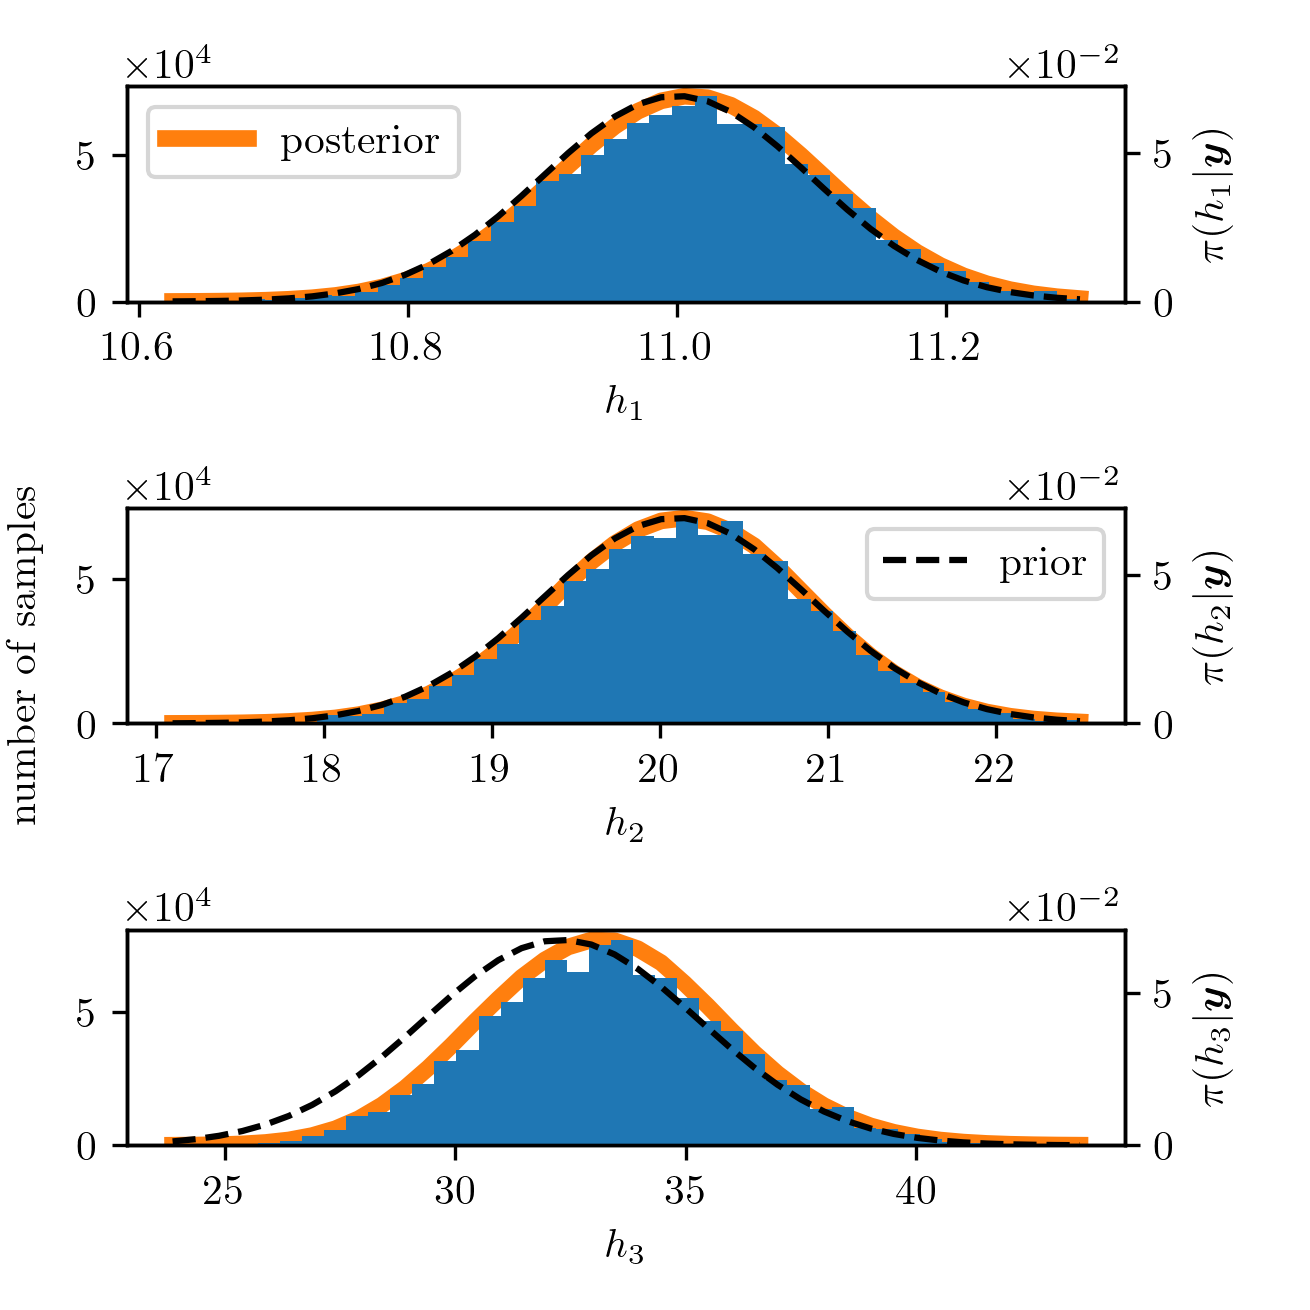
\includegraphics{PHdPTPost0.png}
	\caption[]{}
	\label{fig:}
\end{figure}
\begin{figure}[ht!]
	\centering
	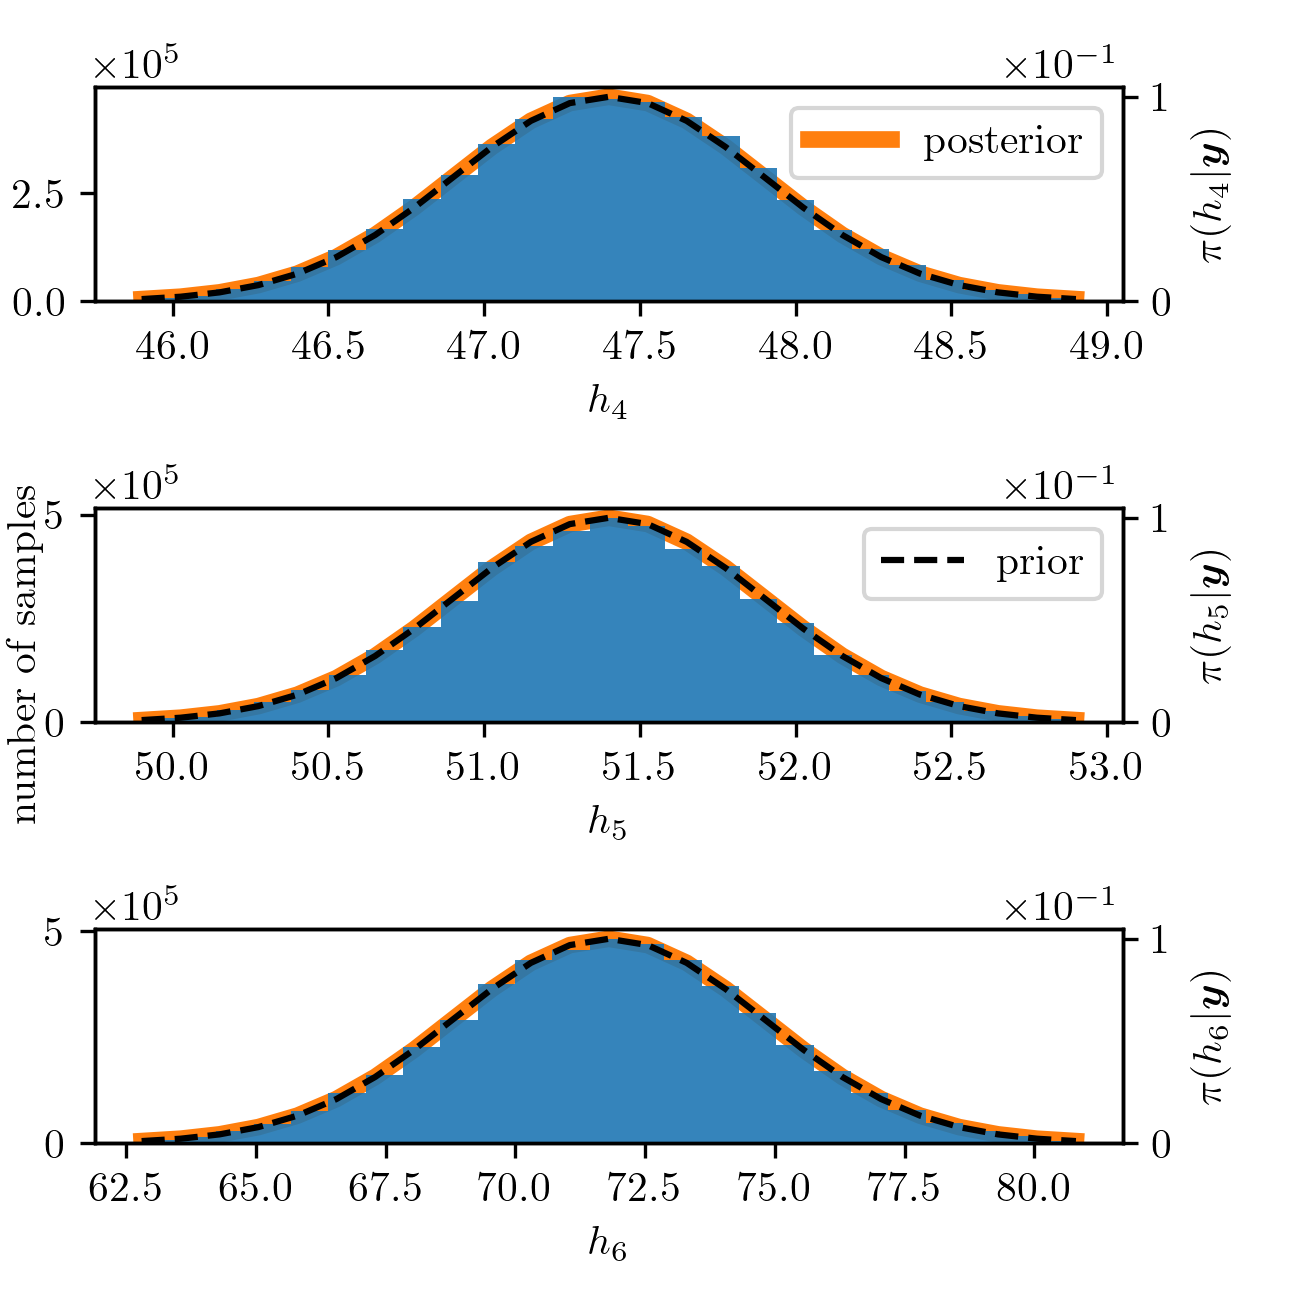
\includegraphics{PHdPTPost1.png}
	\caption[]{}
	\label{fig:}
\end{figure}
\begin{figure}[ht!]
	\centering
	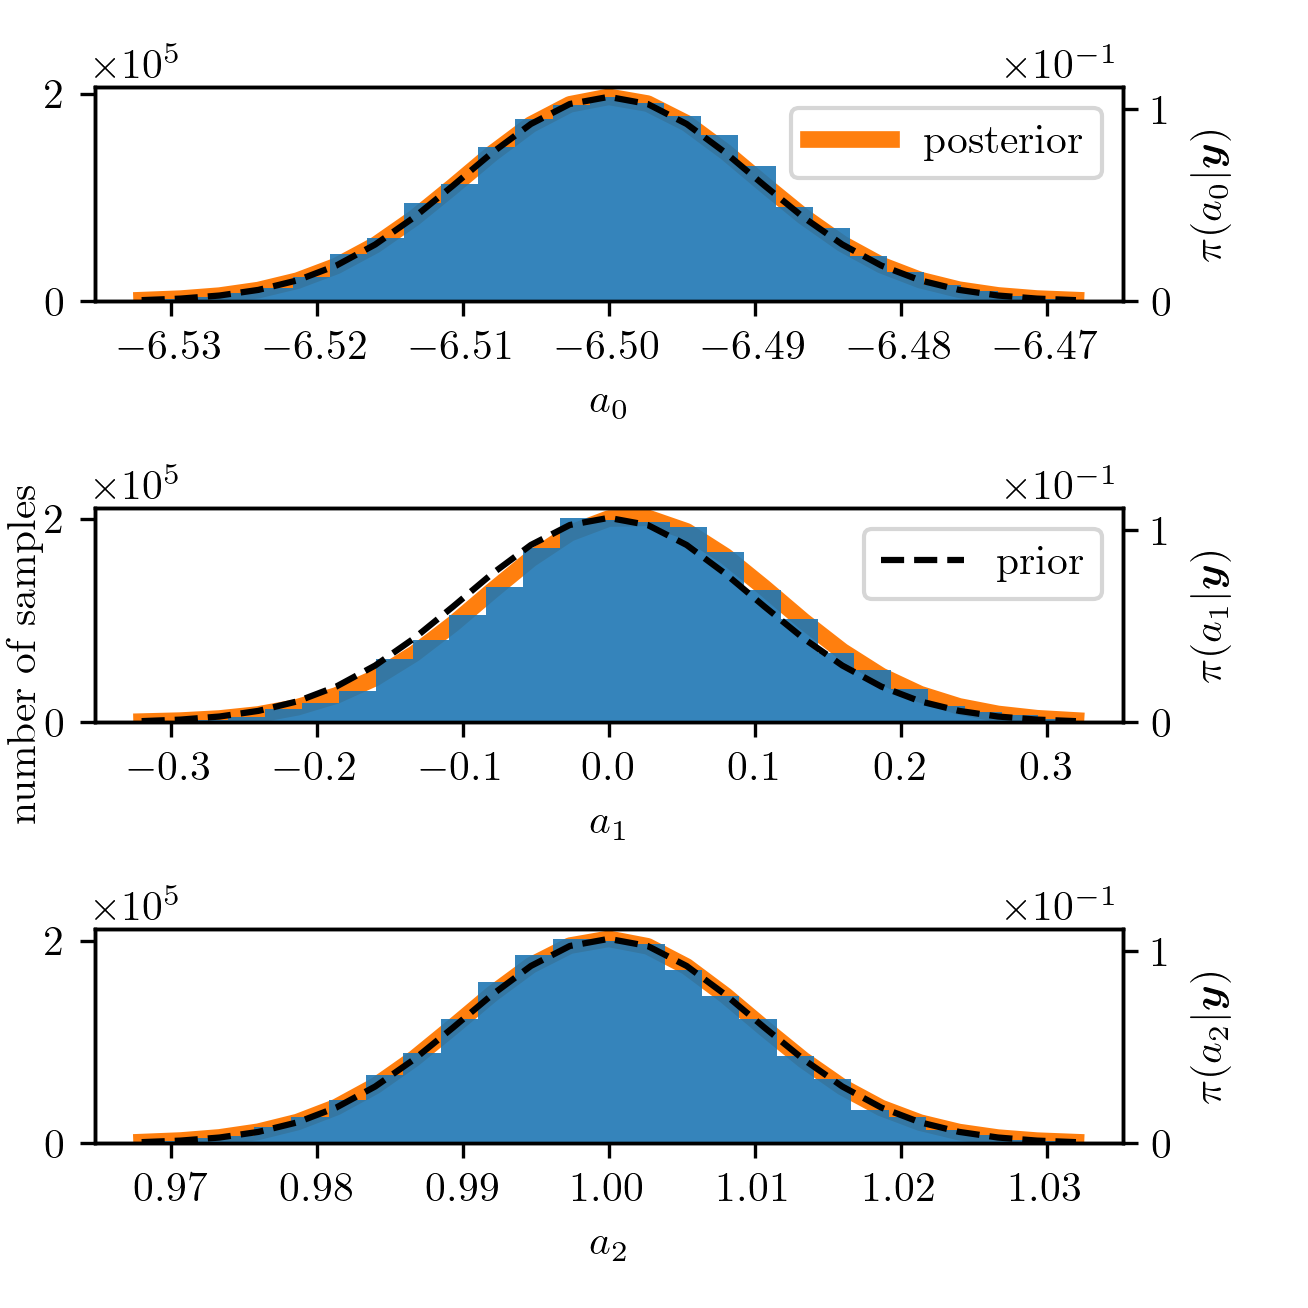
\includegraphics{PHdPTPost2.png}
	\caption[]{}
	\label{fig:}
\end{figure}
\begin{figure}[ht!]
	\centering
	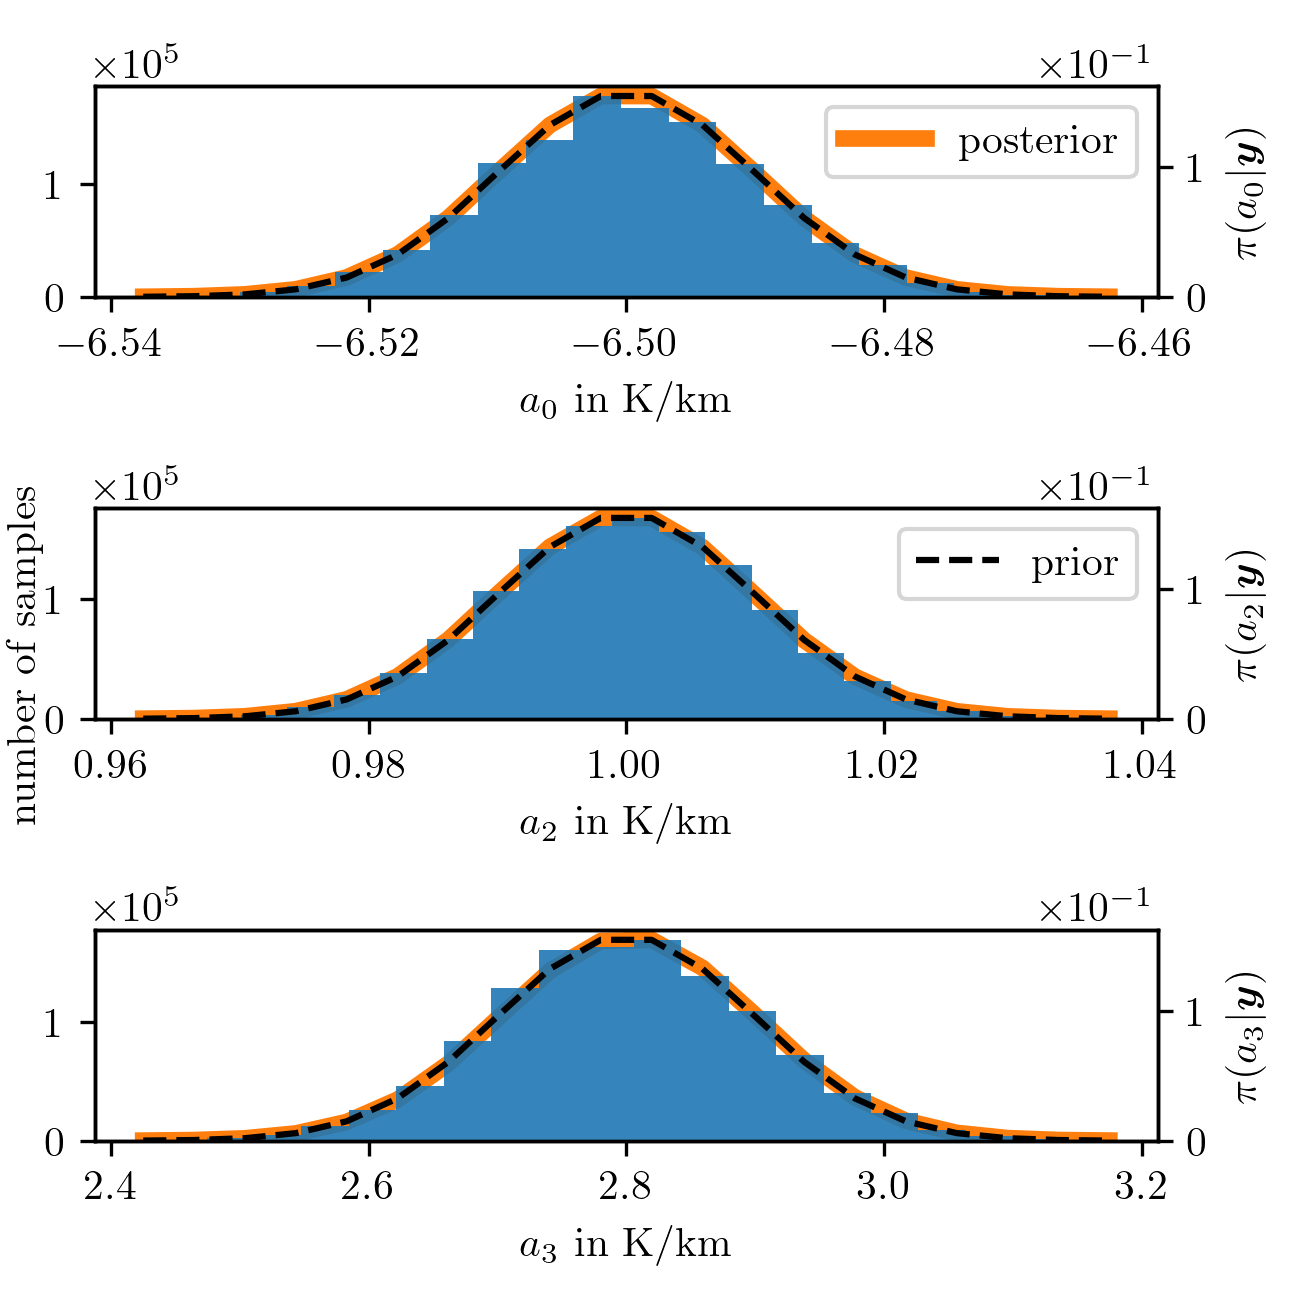
\includegraphics{PHdPTPost3.png}
	\caption[]{}
	\label{fig:}
\end{figure}
\begin{figure}[ht!]
	\centering
	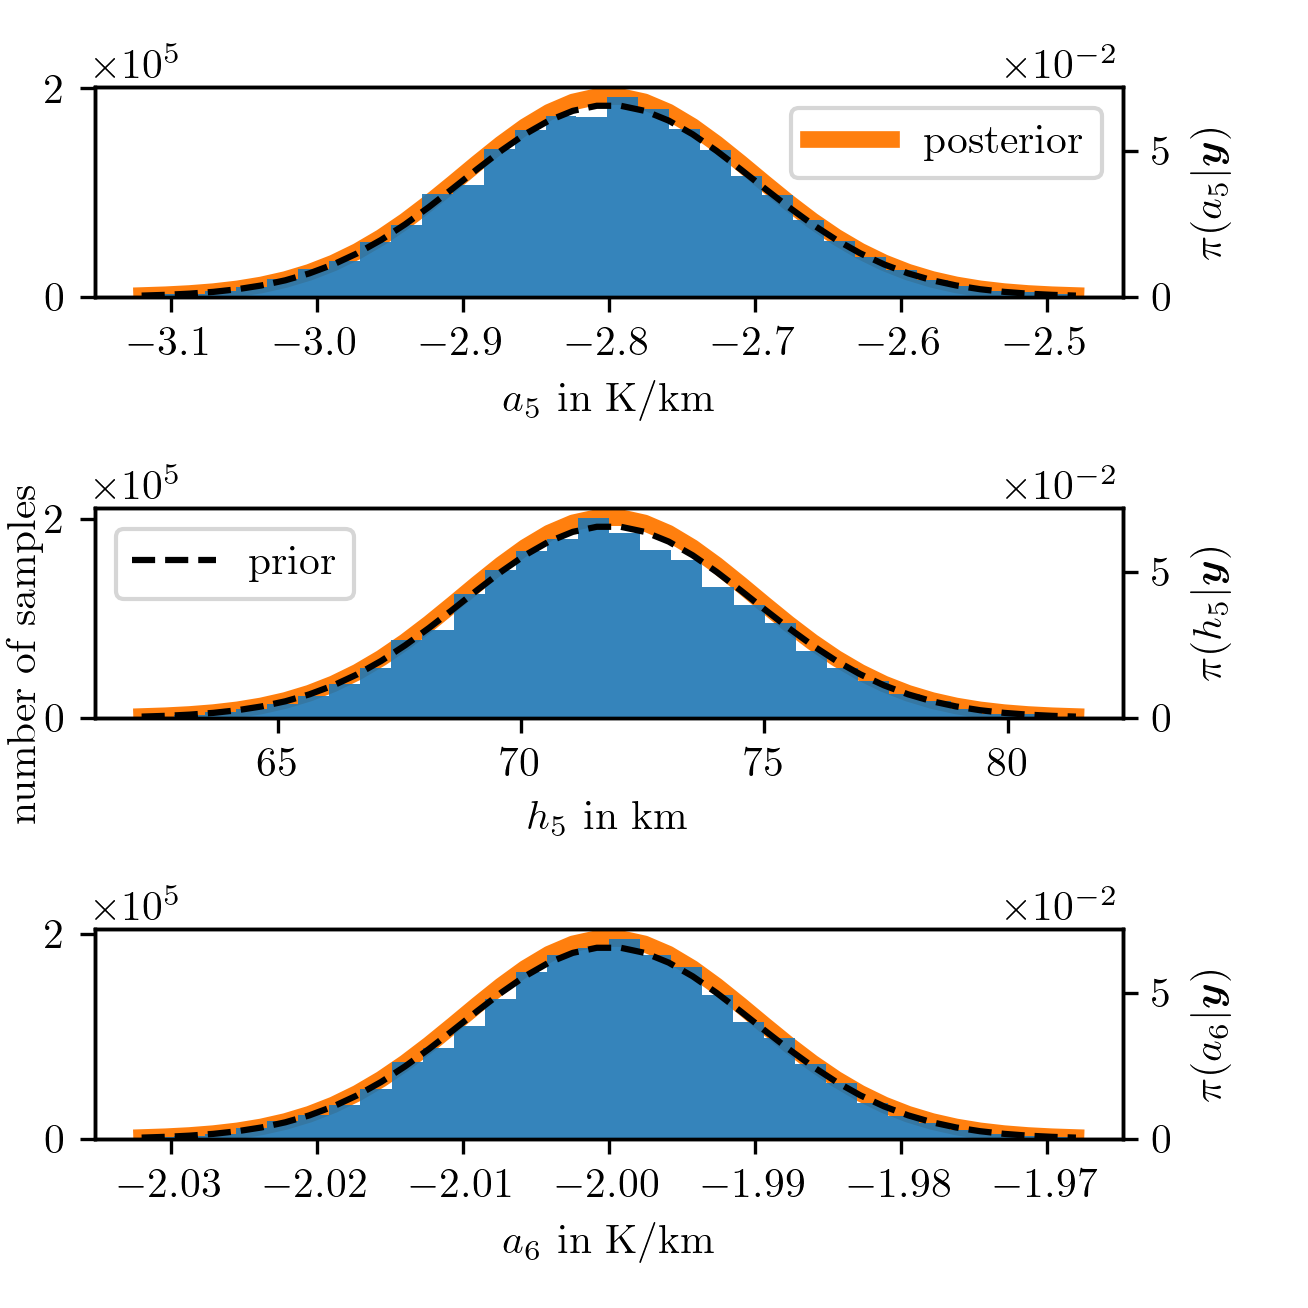
\includegraphics{PHdPTPost4.png}
	\caption[]{}
	\label{fig:}
\end{figure}

\begin{figure}[ht!]
	\centering
	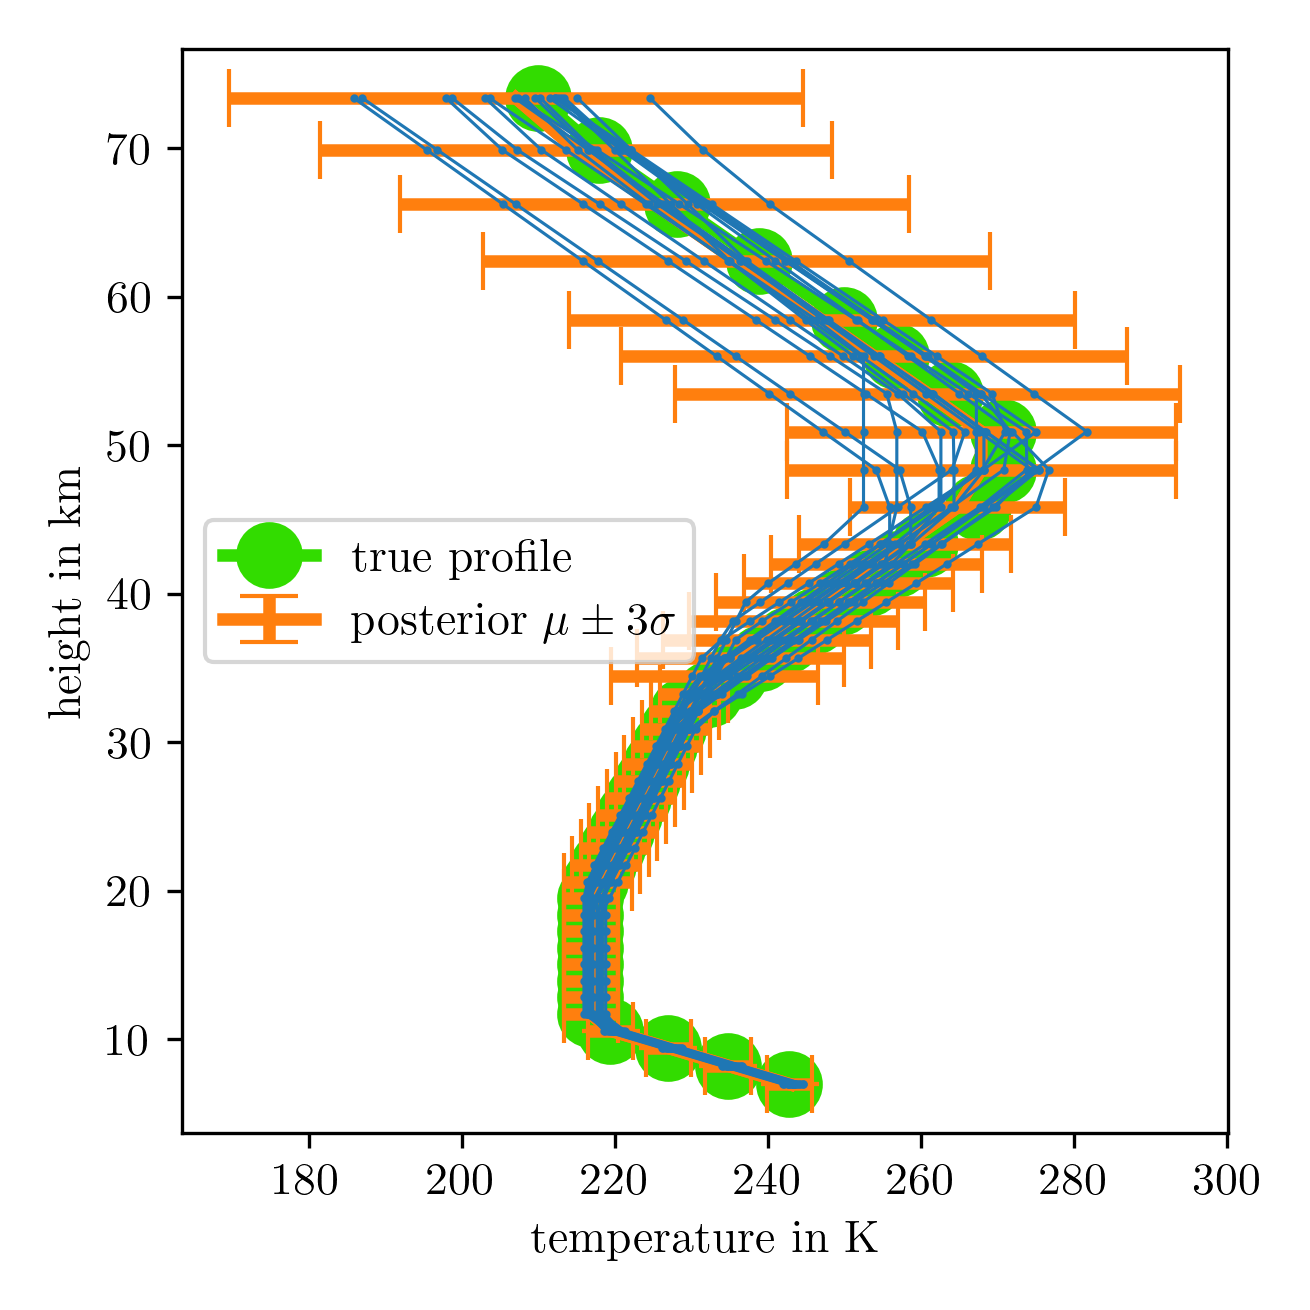
\includegraphics{TempPostMeanSigm.png}
	\caption[]{}
	\label{fig:}
\end{figure}

\begin{figure}[ht!]
	\centering
	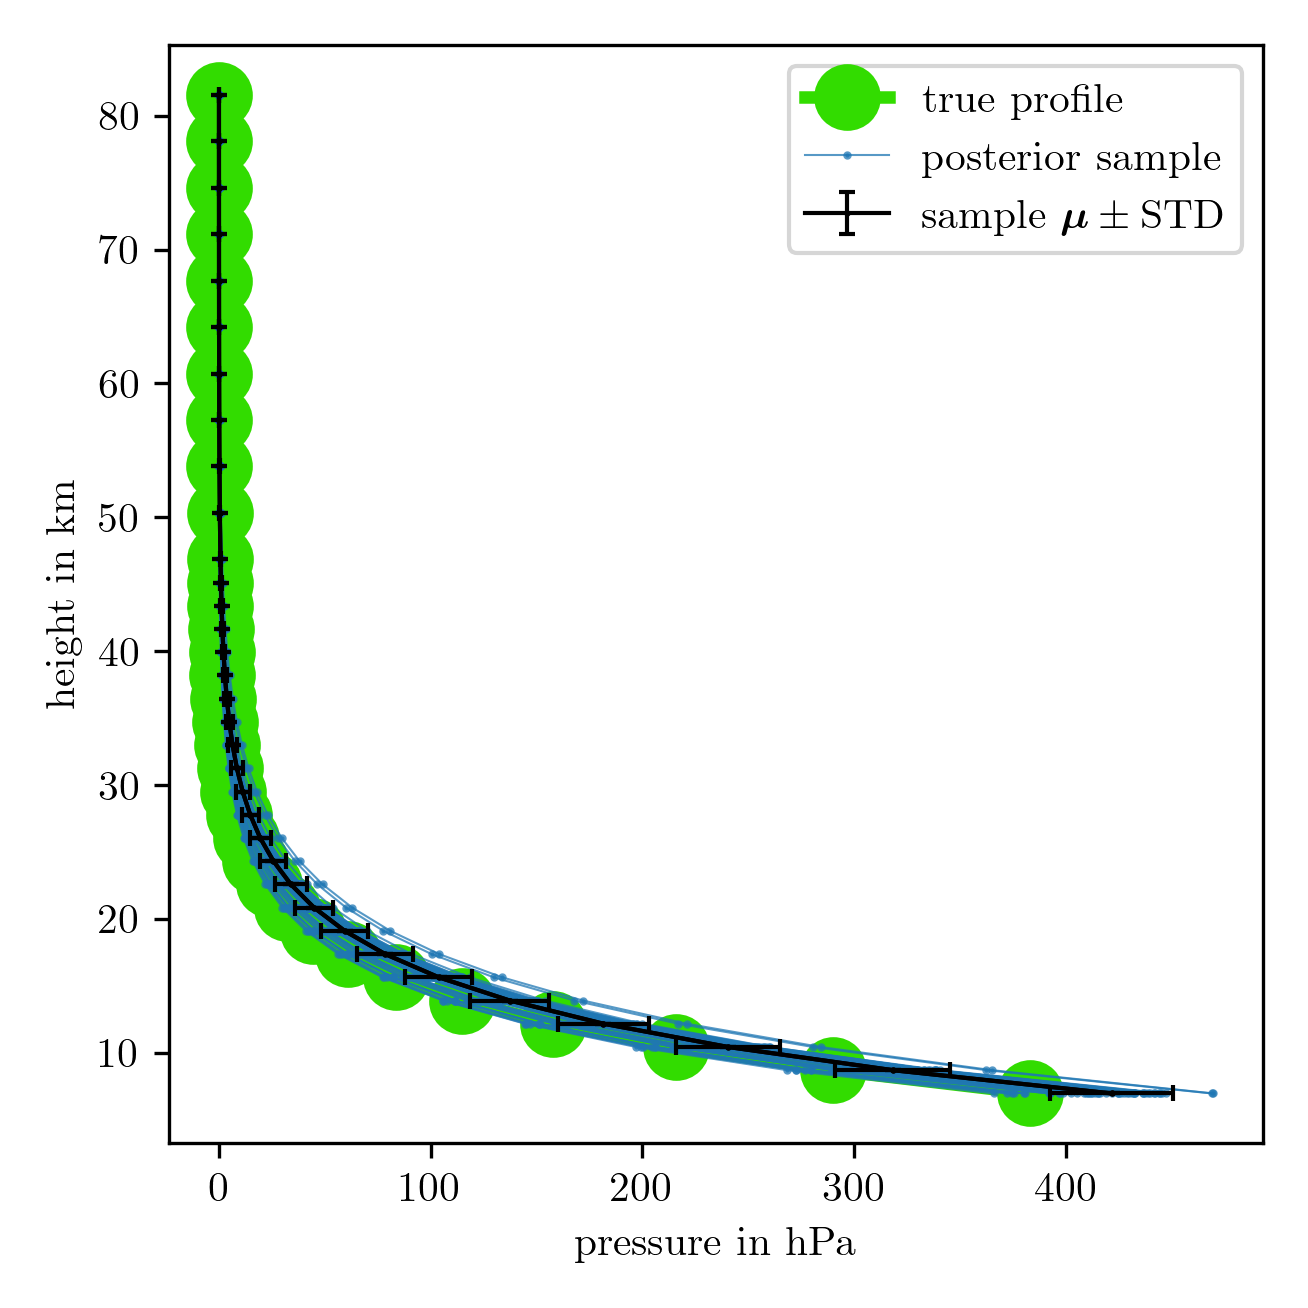
\includegraphics{PressPostMeanSigm.png}
	\caption[]{}
	\label{fig:}
\end{figure}



